\section{Dostupné technologie}
\label{sc:available_technologies}
Aplikace by měla být co nejdostupnější pro běžného uživatele, ideálně by tedy neměla vyžadovat stahování nebo instalaci. Z podstaty této aplikace to ani není potřeba. Jediná výhoda kterou přináší desktopová aplikace je přímý přístup k hardware a lepší výkon, jelikož ale tento typ aplikace nepotřebuje vykreslovat pokročilou 3D grafiku nebo spouštět složité algoritmy, tak je zbytečné se tím zabývat.

Nabízí se tedy webová aplikace nebo mobilní aplikace. Oba typy aplikací se dělí na dvě části, část kterou vidí a se kterou intereaguje uživatel nebo správce, která se nazývá frontend a část která obsluhuje práci s databází, zpracovává požadavky na změny, autorizuje uživatele atd. Jeden backend přitom může obsluhovat frontend jak v podobě webové, tak i mobilní aplikace. Rozdělíme si tedy sekce na \nameref{ss:backend}, \nameref{ss:web} a \nameref{ss:mobile}.

\subsection{Backend}
\label{ss:backend}
Backend tvoří páteř aplikací, zprostředkovává přístup k informacím, umožňuje úpravy a autorizuje uživatele. Z toho důvodu je třeba dbát na kvalitu a bezpečnost kódu. Špatně autorizovaný uživatel, nebo nezabezpečená část databáze je velká bezpečnostní trhlina, které se musí předejít. Nedá se spoléhat na to, že uživatele ověřil frontend, jelikož se s daty na frontendu dá manipulovat (jak na webu, tak i v mobilu), a proto veškeré ověřování probíhá na serveru. Ověřování na frontendu tedy slouží jako čistě estetická záležitost.

Dalším důležitým faktorem je rychlost. Rychlost může ovlivnit několik faktorů, jako je třeba využití složitých algoritmů bez paralelizace, pomalý databázový server, nebo neoptimalizované databázové požadavky.

Při výběru je třeba tedy dbát hlavně na bezpečnost a rychlost. Avšak je třeba zvážit i tzv. code reuse, tedy částečné přepoužití kódu, které muže zjednodušit a zpřehlednit kód aplikace.

\subsubsection*{Javascript}
Javascript je \emph{\uv{otevřený multiplatformní skriptovací jazyk pro tvorbu a přizpůsobení aplikací v podnikových sítích a na internetu}}~\cite{netscapecommunicationscorporation_1995_press}, jako první implementovaný prohlížečem Netscape Navigator 2.0 a rychle adaptován ostatními prohlížeči.

Výhodou je multiplatformnost a jednoduchost vývoje a nasazení. Hlavní nevýhodou je dynamické typovaní, které vede k horší udržitelnosti kódu a odhalení většiny chyb až při běhu aplikace (absence statické kontroly). Tyto neduhy se dají odstranit použitím nějakou syntaktickou nadstavbou, jako je třeba Typescript nebo Flow, které přidávají statické typování proměnných a statickou kontrolu při překladu do Javascriptu.

Javascript se původně vyskytoval jen v prohlížeči, což znamená že nebyl použitelný pro vývoj desktopových a serverových aplikací. To se změnilo s příchodem Node.js. Node.js je prostředí, které umožňuje spouštět javascriptové skripty mimo prohlížeč.

\subsubsection*{Java}
Staticky typovaný, multiplatformní programovací jazyk vycházející z jazyka C, zaštítěný firmou Oracle. Patří mezi nejpopulárnější a nejužívanější programovací jazyky~\cite{stackexchangeinc_2019_stack}. Jeho hlavní užití je právě na straně serveru, a to v kombinaci s frameworkem Spring Boot~\cite{jetbrainssro_2019_demographics}.

\subsubsection*{C\# }
Jazyk velmi podobný Javě, vyvíjený firmou Microsoft. Jeho hlavní nevýhodou byla vysoká závislost na frameworku .NET, který až do příchodu alternativy .NET Core, byl spustitelný pouze na operačním systému Microsoft Windows.

\subsection{Web}
\label{ss:web}
Webová aplikace je pro uživatele nejpřístupnější formou, nemusí nic instalovat, stahovat, pouze otevře prohlížeč s webovou adresou a aplikaci má přístupnou jak na počítači, tak i na mobilu. Nevýhoda oproti mobilní aplikaci je, že vyžaduje přístup k internetu (ne vždy, viz~\hyperref[sss:pwa]{PWA}).

\subsubsection*{Javascript}
\label{ss:javascript}
Pro vývoj webové aplikace lze v Javascriptu zvolit z mnoha možností, ať už co se týče syntaktické nadstavby (Typescript, Flow), nebo knihoven a frameworků. Jelikož jich je velké množství, tak si jen stručně probereme tři nejpopulárnější a to React, Angular a Vue~\ref{fig:popularity_plot}.

React je knihovna vyvíjená společností Facebook, která ho sama využívá pro tvorbu jejich aplikací, např Facebook nebo Messenger. Jeho hlavní výhodou je, možnost si spoustu věcí přizpůsobit k vlastní potřebě (např. routing, globalní uložiště dat, \ldots{}), což mimo jiné vede k menší velikosti výsledné aplikace a vyšší rychlosti. React sám o sobě není ani závislý na prohlížeči a může být využit např. pro vývoj aplikace spouštěné z příkazové řádky.

Angular je framework od společnosti Google, taktéž využívaný v řadě aplikací. Hlavní výhodou je, že nabízí téměř vše co může programátor potřebovat, díky čemuž nemusí řešit občasné potíže s kompatibilitou knihoven jako u Reactu, ale na druhou stranu je výsledná aplikace větší a pomalejší, jelikož obsahuje i nevyužívané funkce.

Vue je knihovna velmi podobná Reactu, sdílí spolu velkou část ideologií~\cite{you_2014_comparison}, ale Vue se zaměřuje na projekty malé až střední a React in na ty velké. Výhoda tedy je rychlost a jednoduchost, nevýhoda je, že s rostoucím projektem a týmem se projekt stává méně přehledný a udržovatelný.

\begin{figure}[h!]
    \centering
    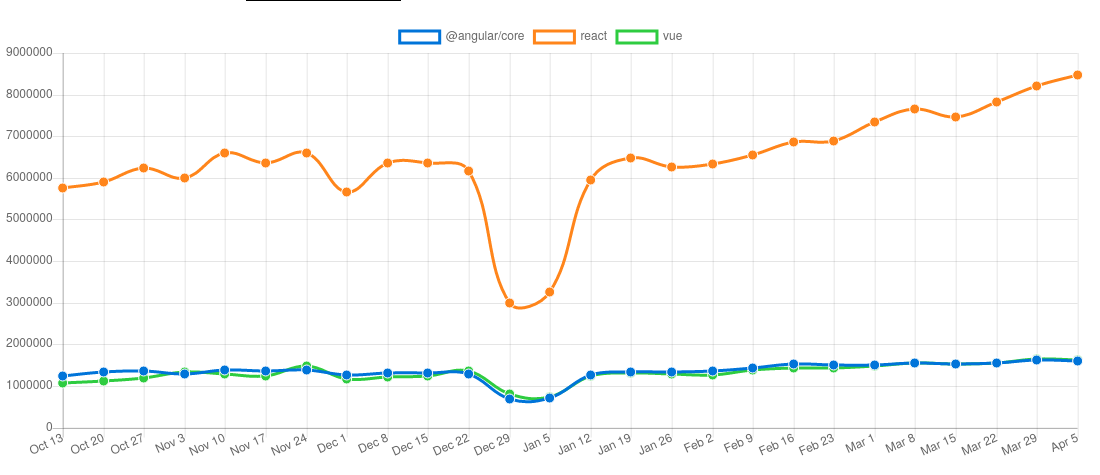
\includegraphics[width=\textwidth]{assets/popularity_plot.png}
    \caption{Popularita Javascriptových frameworků}
    \label{fig:popularity_plot}
    \textit{Zdroj:}~https://www.npmtrends.com/@angular/core-vs-react-vs-vue
\end{figure}

\subsubsection*{C\# }
V C\# se dá vyvíjet i frontend a to za pomoci frameworku ASP.NET, který závisí na frameworku .NET. V dnešní době se na nové projekty již příliž nevyužívá. Lze jej využít v kombinaci s Javascriptem a jeho knihovnami. Největší výhoda tohoto přístupu je striktní dodržení přístupu Model-View-Controler, nevýhodou jsou vyšší nároky na znalost obou technologií, což pro juniorního programátora může být problém.

\subsection{Mobil}
\label{ss:mobile}
Mobilním technologiím se budeme v této práci zabývat jen okrajově, protože cílem práce je webová aplikace. Přesto je jistá možnost jak z webové aplikace vytvořit aplikaci mobilní nebo z nějaké části sdílet kód mezi webovou a mobilní aplikací.

\subsubsection*{Responzivní webová aplikace}
\label{sss:responsive_web_app}
První a nejjednodušší možností jak vytvořit mobilní aplikaci je pouze optimalizovat aplikaci webovou tak, aby se dala prohlížet i na mobilu. Hlavní výhodou je nízká náročnost vývoje takové aplikace (v porovnání s tvorbou celé mobilní aplikace), nevýhodou však je, že aplikace nemá přístup k některým částem zařízení, třeba stavu baterie, gyroskopu, poloze a dalším.

\subsubsection*{Progressive Web App}
\label{sss:pwa}
Progressive Web App, nebo Progresivní Webová Aplikace, je způsob jak z webové aplikace udělat aplikaci mobilní bez nutnosti vytvářet nativní aplikaci. Tento způsob je kombinací \hyperref[sss:responsive_web_app]{resonzivní webové aplikace}, manifestu a service workeru. Manifest je soubor udávající informace pro mobilní prohlížeč, jak se aplikace má jmenovat, popis, ikony, barevné schéma, autor atd. Jedná se o obdobu manifestu, který mají mobilní aplikace. Service worker je speciální skript, který běží na pozadí a umožňuje načítat data, přistupovat k notifikacím nebo poloze (na mobilu i webu) atd. V případě, že webová aplikace splňuje všechny zmíněné náležitosti, a uživatel vstoupí na web pomocí jednoho z prohlížečů, které podporují \hyperref[sss:pwa]{PWA}, pak má možnost si tu aplikaci přidat na plochu mobilu a spouštět stejně jako nainstalovanou aplikaci. Takto nainstalovaná aplikace funguje i bez přístupu k internetu, ale je to v podstatě stažený web spustěný v prohlížeči. Hlavní nevýhodou je absence možnosti práce přímo s hardwarem telefonu, takže to není vhodné např. pro mobilní hry. Dalším problémem je podpora na zařízeních s operačním systémem iOS. Ačkoliv je společnost Apple původním tvůrcem této myšlenky~\cite{ritchie_2018_app}, tak aplikace na iOS nemají přístup k tolika informacím a možnostem jako ty na Androidu a jsou tedy limitované.

\subsubsection*{Hybridní aplikace}
Hybridní aplikace jsou posledním mezikrokem mezi mobilní a webovou aplikací. Jedná se o aplikaci webovou, která je později zkompilovaná i s jádrem prohlížeče a může být přidaná na Android Play Store, resp. iOS App Store. Takto vytvořená aplikace má již přístup ke všem částem telefonu, stejně jako aplikace nativní, ale nevýhoda je velikost balíčku potažmo aplikace. Ta v sobě obsahuje i část prohlížeče a aplikace má vyšší nároky na paměť a procesorový čas.

\subsubsection*{Nativní aplikace}
Poslední kategorie jsou aplikace nativní, tedy přímo určené pouze na mobilní zařízení. Existuje mnoho programovacích jazyků, které lze při vývoji použít, ať už to je Java a Kotlin pro Android nebo Objective C a Swift pro iOS. Hlavní nevýhoda tedy je mnohem více práce a potenciálně duplicitní kód. Z toho důvodu existují různé multiplatformní frameworky, které tyto neduhy řeší.

V rámci této práce si zmíníme pouze React Native. Jedná se o framework syntaxem velmi podobný frameworku ReactJS a důvod proč zmínit zrovna tento a ne ostatní, je možnost přepoužití kódu z webové aplikace. Jisté části aplikace napsané v ReactJS lze bez úpravy použít i v React Native a obráceně. Tedy aplikace psaná za použití React Native má stejné benefity jako aplikace nativní, ale zároveň v ní lze přepoužít části aplikace webové. Příklad takového přepoužití je zde~\cite{sepulveda_2017_share}.

Toto přepoužití vyplývá z architektury samotného Reactu, kde React je knihovna které zpracovává vstupy, ovládá stav aplikace, kontroluje změny a generuje výstupy. Následně na řadu přichází tzv. \uv{Renderer}, který funguje jako rozhraní mezi platformou (web, mobil, konzole, \ldots{}) a Reactem. U webu je tímto rozhraním knihovna \uv{React-DOM} a u mobilu právě \uv{React Native}.

